\documentclass[border=8pt]{standalone}
\usepackage{pgfplots}
\pgfplotsset{compat=1.18}
\begin{document}
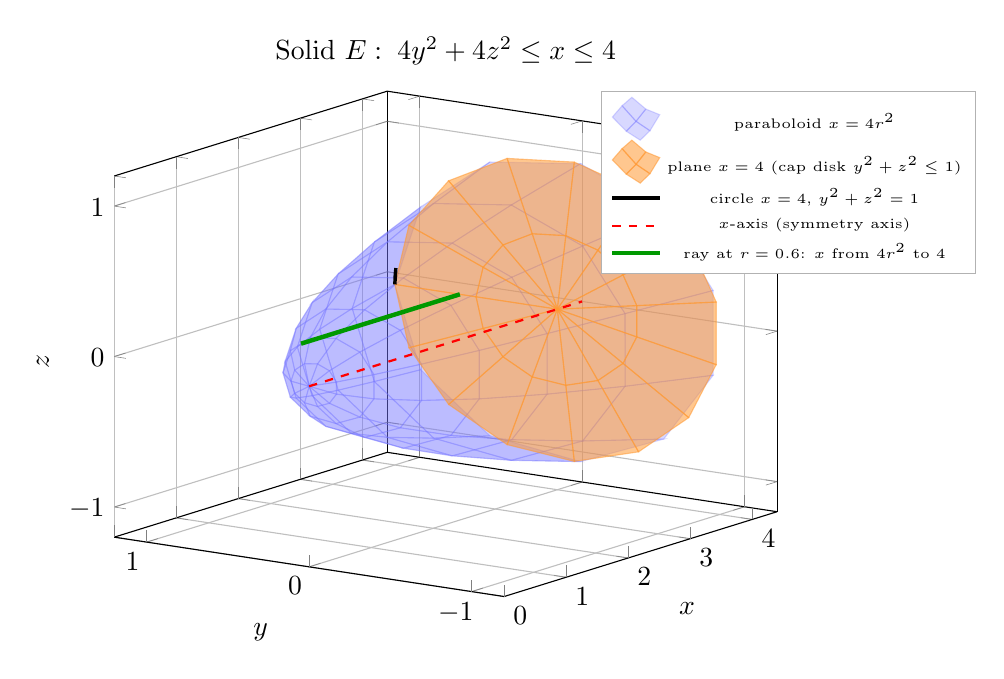
\begin{tikzpicture}
\begin{axis}[view={-55}{16}, width=10cm, height=8cm,
    xlabel={$x$}, ylabel={$y$}, zlabel={$z$},
    xmin=0, xmax=4.4, ymin=-1.2, ymax=1.2, zmin=-1.2, zmax=1.2,
    xtick={0,1,2,3,4}, ytick={-1,0,1}, ztick={-1,0,1},
    grid=major,
    title={Solid $E:\;4y^{2}+4z^{2}\leq x\leq 4$},
    legend style={font=\tiny, at={(1.30,1.0)}, anchor=north east, draw=black!30, fill=white}]
    \addplot3[surf, blue!55, opacity=0.28, shader=flat,
          domain=0:1, domain y=0:6.283, samples=8, samples y=12]
   ({4*x^2}, {x*cos(deg(y))}, {x*sin(deg(y))});
   \addlegendentry{paraboloid $x=4r^2$}
    \addplot3[surf, orange!80, opacity=0.55, shader=flat,
          domain=0:1, domain y=0:6.283, samples=3, samples y=16]
   ({4}, {x*cos(deg(y))}, {x*sin(deg(y))});
   \addlegendentry{plane $x=4$ (cap disk $y^2+z^2\leq1$)}
    \addplot3[black, very thick, domain=0:6.283, samples=48] ({4},{cos(x)},{sin(x)});
   \addlegendentry{circle $x=4$, $y^2+z^2=1$}
    \addplot3[red, dashed, thick] coordinates {(0,0,0) (4.4,0,0)};
   \addlegendentry{$x$-axis (symmetry axis)}
    \addplot3[green!60!black, ultra thick] coordinates {(1.44,0.6,0) (4,0.6,0)};
   \addlegendentry{ray at $r=0.6$: $x$ from $4r^2$ to $4$}
\end{axis}
\end{tikzpicture}
\end{document}
